\documentclass{sig-alternate-05-2015}
\usepackage[brazilian]{babel}
\usepackage[utf8]{inputenc}
\usepackage[T1]{fontenc}

\usepackage{graphics}

\begin{document}

%Conference

%
% --- Author Metadata here ---
%\CopyrightYear{2007} % Allows default copyright year (20XX) to be over-ridden - IF NEED BE.
%\crdata{0-12345-67-8/90/01}  % Allows default copyright data (0-89791-88-6/97/05) to be over-ridden - IF NEED BE.
% --- End of Author Metadata ---

\title{Assignment 1 - Implementation of a Crawler}
%
% You need the command \numberofauthors to handle the 'placement
% and alignment' of the authors beneath the title.
%
% For aesthetic reasons, we recommend 'three authors at a time'
% i.e. three 'name/affiliation blocks' be placed beneath the title.
%
% NOTE: You are NOT restricted in how many 'rows' of
% "name/affiliations" may appear. We just ask that you restrict
% the number of 'columns' to three.
%
% Because of the available 'opening page real-estate'
% we ask you to refrain from putting more than six authors
% (two rows with three columns) beneath the article title.
% More than six makes the first-page appear very cluttered indeed.
%
% Use the \alignauthor commands to handle the names
% and affiliations for an 'aesthetic maximum' of six authors.
% Add names, affiliations, addresses for
% the seventh etc. author(s) as the argument for the
% \additionalauthors command.
% These 'additional authors' will be output/set for you
% without further effort on your part as the last section in
% the body of your article BEFORE References or any Appendices.

\numberofauthors{4} %  in this sample file, there are a *total*
% of EIGHT authors. SIX appear on the 'first-page' (for formatting
% reasons) and the remaining two appear in the \additionalauthors section.
%
\author{
% You can go ahead and credit any number of authors here,
% e.g. one 'row of three' or two rows (consisting of one row of three
% and a second row of one, two or three).
%
% The command \alignauthor (no curly braces needed) should
% precede each author name, affiliation/snail-mail address and
% e-mail address. Additionally, tag each line of
% affiliation/address with \affaddr, and tag the
% e-mail address with \email.
%
% 1st. author
\author XYuri Niitsuma\\
       \affaddr{Universidade Federal de Minas Gerais}\\
       \email{yuriniitsuma@dcc.ufmg.br}
\and  % use '\and' if you need 'another row' of author names
}
% There's nothing stopping you putting the seventh, eighth, etc.
% author on the opening page (as the 'third row') but we ask,
% for aesthetic reasons that you place these 'additional authors'
% in the \additional authors block, viz.
\date{19 November 2017}
% Just remember to make sure that the TOTAL number of authors
% is the number that will appear on the first page PLUS the
% number that will appear in the \additionalauthors section.

\maketitle
% \begin{abstract}
%
% \end{abstract}
\section{Introdução} O trabalho consiste em criar um crawler que coletará
links (internos e externos) e criará um arquivo de dump contendo a url e a
página em html conforme está na especificação.

Alguns requisitos do crawler são:



\begin{itemize}
  \item{Formato do arquivo de dump:}

  |||<url>|<conteúdo>|||<url>|<conteúdo>|||...

  |||<url>|<conteúdo>|||


  \item{Código em C++}
  \item{Uso da biblioteca Chilkat é recomendado}
  \item{Baixar páginas no domínio *.br}
  \item{Coletar somente páginas HTML}
  \item{Coletar páginas com no máximo 2 MB}
  \item{Mínimo: 1 milhão de páginas}
  \item{Máximo: 5 milhões de páginas}
  \item{Comprimir o arquivo final no formato .tar}
\end{itemize}

Todos os requisitos foram atendidos com exceção do mínimo da
coleção de páginas que será explicado a seguir.

\section{Implementação}

O trabalho se iniciou em aprender como o framework Chilkat funciona criando os arquivos `spider.cpp` e `spider.h`.

Cada instância do Spider foi criado para ficar responsável por apenas um dommínio. Para evitar detecção de DDoS e tentar acessar mais páginas paralelamente.

O arquivo `main.cpp` é o que gerencia todo o processo, em que instância os \textit{spiders} e faz o escalonamento para enviar o máximo determinado de threads a cada iteração.

Para facilitar o \textit{DEBUG} (estou entregando o trabalho atrasado por causa disto xD), o escalonador é feito em cada iteração (\textit{short-term scheduler}). Quando determinado é disparado as threads responsável pra cada domínio e depois é esperado que as threads terminem para que coletem os links para criar outras threads de domínio e os guardam em arquivos temporários caso o programa pare. Como é ilustrado na figura \ref{fig1}.

\begin{figure}
  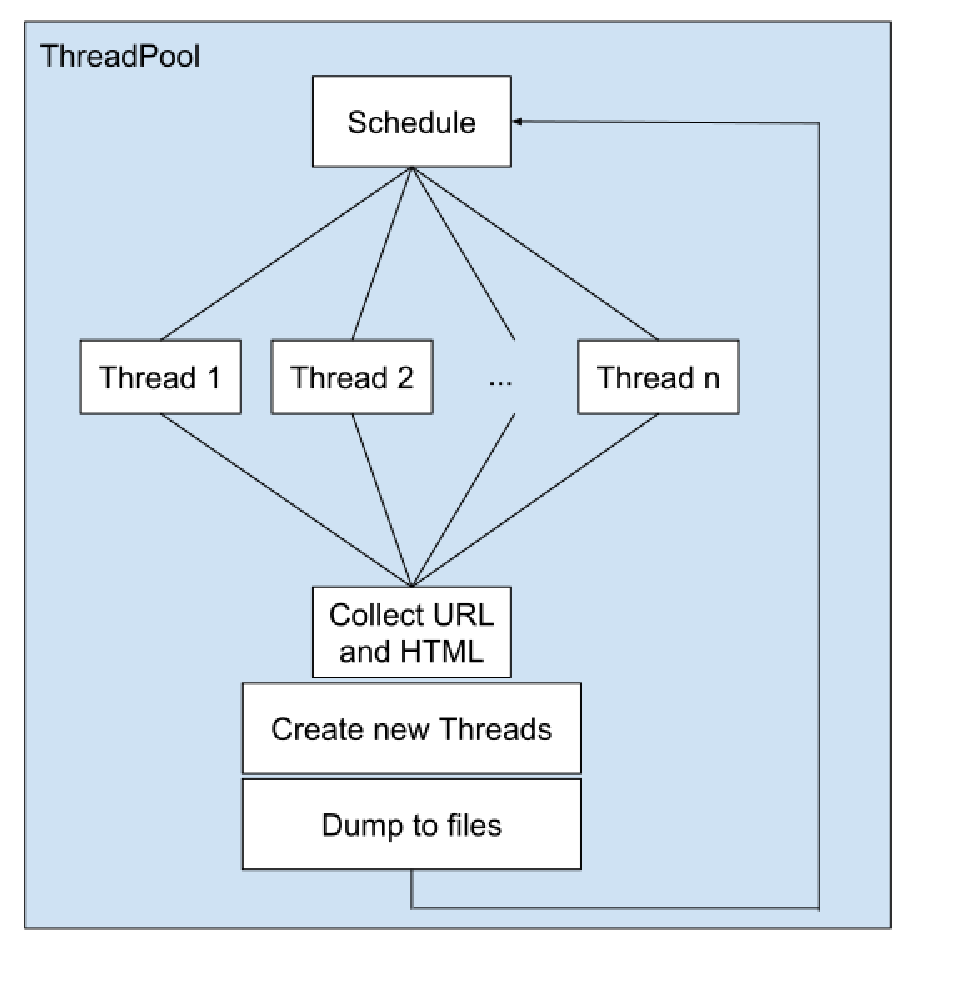
\includegraphics[width=0.6\textwidth]{images/aux1.eps}
  \caption{ThreadPool}
  \label{fig1}
\end{figure}

Portanto, um thread pode criar um gargalo, mas está setado o timeout para 10 segundos.

A fila utilizada contendo os theads para serem disparados é FIFO.

\subsection{Arquivos temporários}
Os arquivos temporários criados são:

\begin{itemize}
  \item output\_file.txt

  Arquivo contendo dump das urls e páginas html

  \item save\_state.sav

  Arquivo guarda todas as urls que estão na lista no final da iteração. Caso o programa é reiniciado, ele carrega todas as urls para que entre na fila novamente.

  \item unique\_id\_file.txt

  Coleção de hashs em \textit{unsigned long long}, calculado com \textbf{URL + HTML}, assim é detectado se uma página já foi acessada e assim ignorada. E páginas atualizadas como \textbf{g1.globo.com} são novamente acessadas.

\end{itemize}

Lembrando que o comando `make clean` deleta o conteúdo destes arquivos.

\section{Utilização}

O \textbf{Makefile} é composto apenas por:

\begin{itemize}
  \item \textbf{make}: compila
  \item \textbf{make run}: roda o programa, se conter arquivos temporários, ele o carrega o estado a partir e adiciona todos a \textbf{UnspideredLinks}.
  \item \textbf{make clean}: apaga os arquivos temporários inclusive o dump das \textbf{URLs + HTMLs}.
\end{itemize}

Segue uma imagem do programa em utilização:

\begin{figure}[h]
  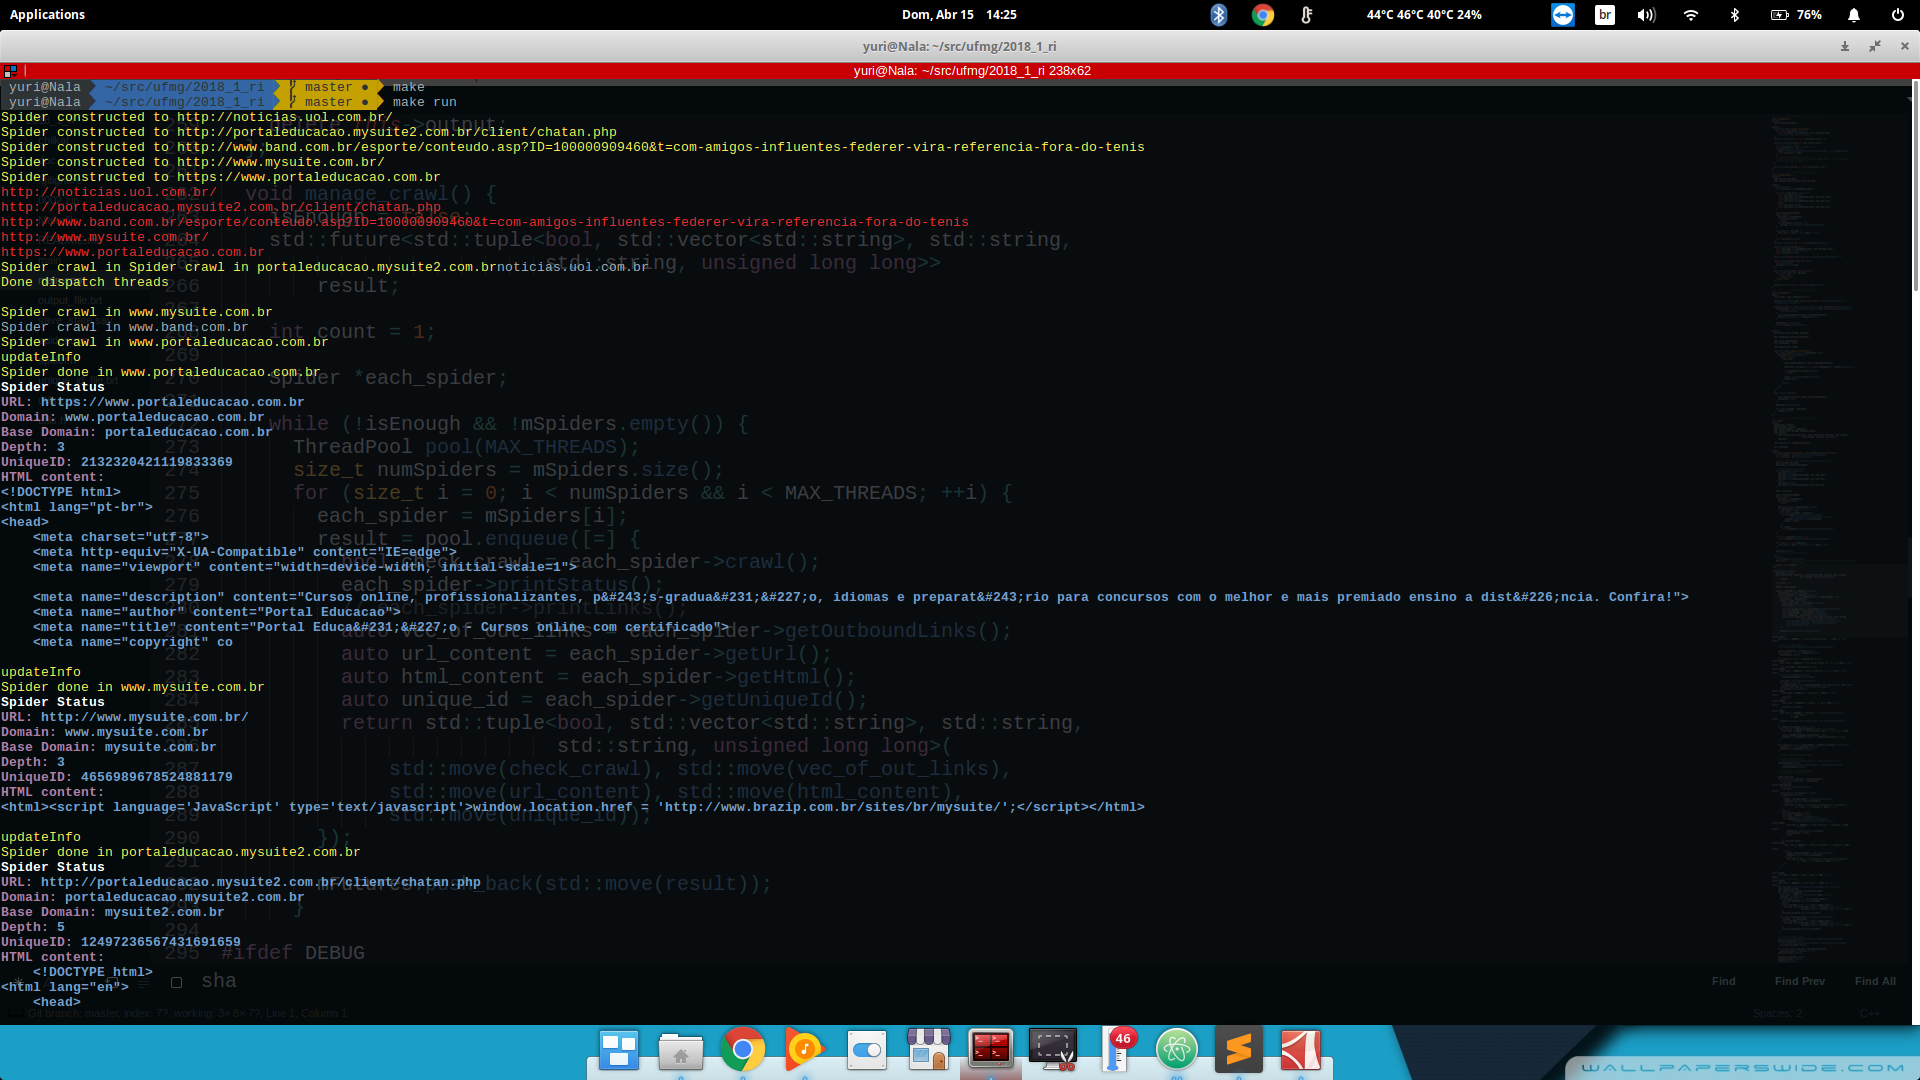
\includegraphics[width=0.5\textwidth]{images/aux2.png}
  \caption{Programa sendo executado}
  \label{fig2}
\end{figure}

Aqui é imprimido a inicialização dos spiders é o que cada spider coletou:

Exemplo:
\begin{itemize}
  \item \textbf{URL}: https://www.portaleducacao.com.br
  \item \textbf{Domain}: www.portaleducacao.com.br
  \item \textbf{Base Domain}: portaleducacao.com.br
  \item \textbf{Depth}: 3

  Profundidade da URL

  \item \textbf{UniqueID}: 2132320421119833369

  ID único para identificar se esta página já foi coletada.

  \item \textbf{HTML content}:

  Conteúdo HTML da página.
\end{itemize}

\section{Resultados}

A implimentação utilizando ThreadPools foi dedcidida pois é a mais fácil de encontrar bugs, pois a cada iteração de disparo é feito a sincronização e a escrita em dados. Houve várias tentativas de manter totalmente em paralelo, mas ão consegui encontrar problemas de sincronia em escrita de arquivos.

Além do \textit{tradeoff} do atraso do trabalho teve o problema do gargalo. Por exemplo nas figuras \ref{fig3} e \ref{fig4}.

\begin{figure}
  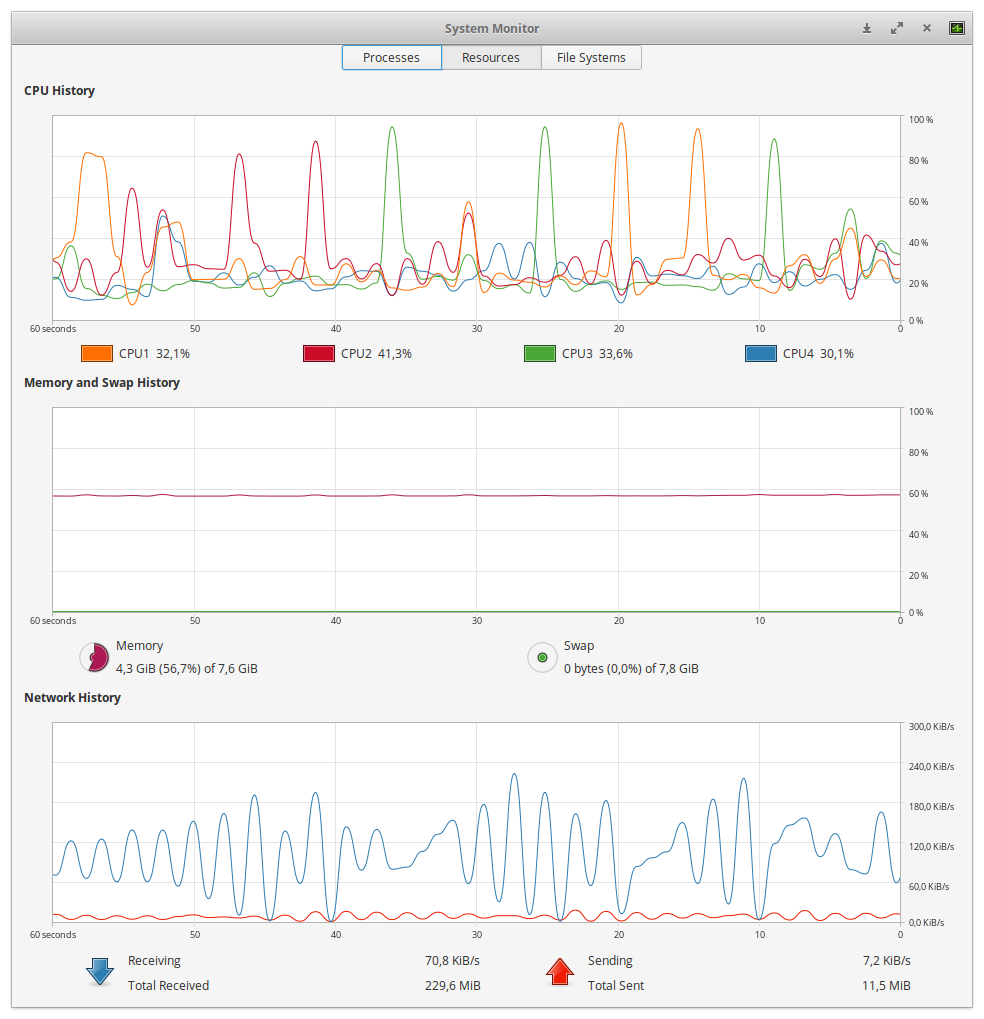
\includegraphics[width=0.5\textwidth]{images/monitor.png}
  \caption{Uso de CPU, RAM e Rede no início}
  \label{fig3}
\end{figure}

Em que após algumas iterações ocorrem atrasos que não foram possíveis serem sanados.

Os possíveis erros são:

\begin{itemize}
  \item complexidade de links colectados no Spider
  \item má utilização da classe vector do cpp
  \begin{itemize}
    \item muitos \textbf{inserts} e \textbf{erase} utilizados
  \end{itemize}
\end{itemize}

\begin{figure}
  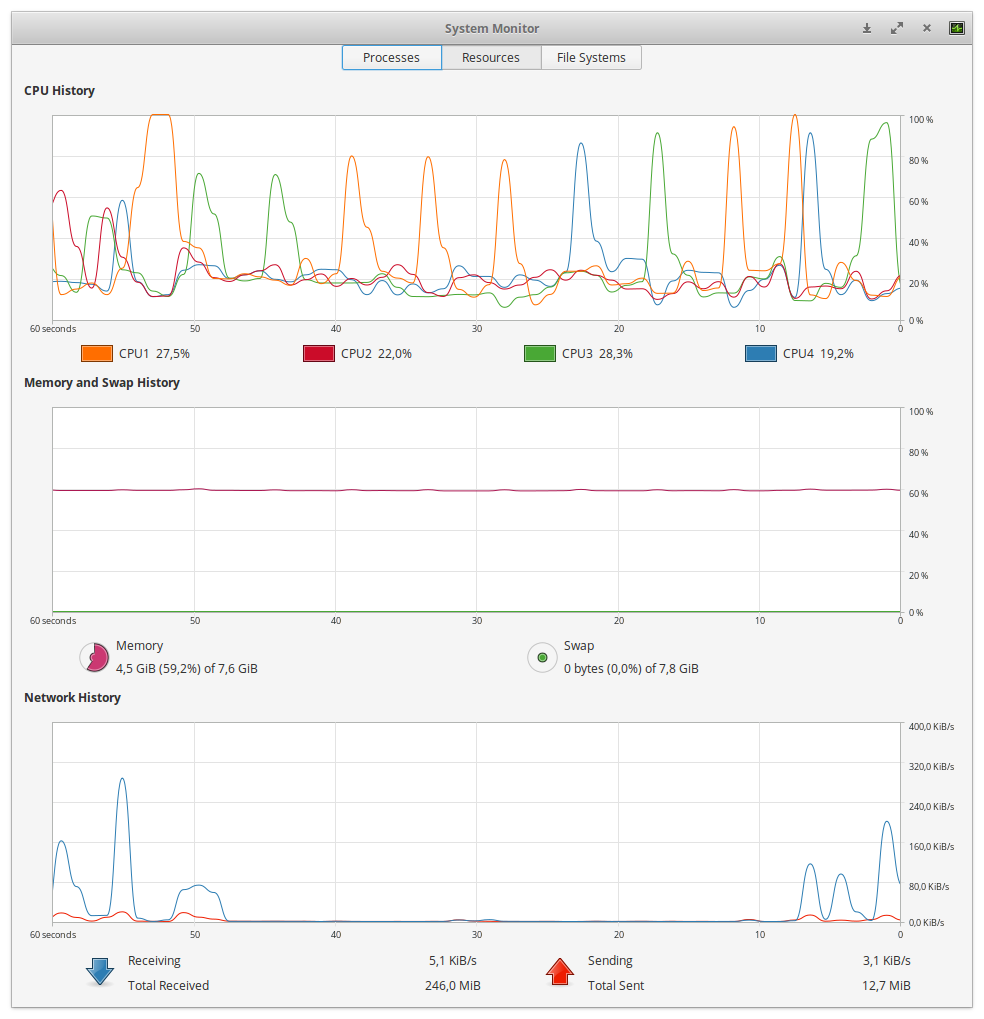
\includegraphics[width=0.5\textwidth]{images/monitorwithgargalo.png}
  \caption{Uso de CPU, RAM e Rede com gargalo}
  \label{fig4}
\end{figure}

\subsection{Coleção}

A quantidade de páginas coletadas foram \textbf{27114} páginas, através dos UniqueIDs criados, e o dump da coleção foi de \textbf{2,9GB}. Que considerado bem pouco, mas foi ocasionado pelo uso de detecção de UniqueIDs e ciclos no grafo da Web que eu não consegui sanar (afinal, era desejado baixar sites que são atualizados depois de um tempo).

O crescimento da coleção se tornou logarítmica, pois depois de uma hora já continha 1GB, mas no final do dia foi coletado no total de 2GB.

\begin{figure}[h]
  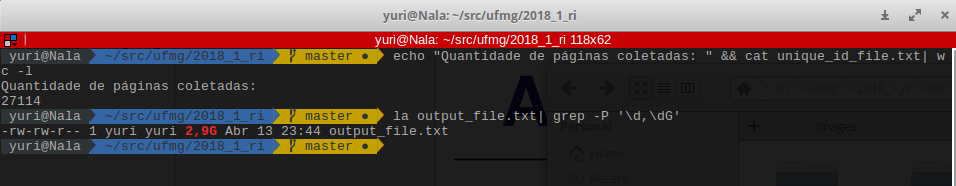
\includegraphics[width=0.5\textwidth]{images/sizecollected.png}
  \caption{Quantidade de páginas coletadas}
  \label{}
\end{figure}


\newpage
% \section{Conclusão}

Neste trabalho utilizamos conhecimento base de teoria da informação e teoria de decisão para escolher as melhores estratégias de investimento em ações durante períodos de tempo.
Através de definições matemáticas é possível encontrar a melhor estratégia apesar do sistema ser estocástico e iterativo.

%\end{document}  % This is where a 'short' article might terminate
%
% The following two commands are all you need in the
% initial runs of your .tex file to
% produce the bibliography for the citations in your paper.
% \bibliographystyle{abbrv}
% \bibliography{sigproc}  % sigproc.bib is the name of the Bibliography in this case

% You must have a proper ".bib" file
%  and remember to run:
% latex bibtex latex latex
% to resolve all references
%
% ACM needs 'a single self-contained file'!
%
%APPENDICES are optional
%\balancecolumns
\end{document}
